\chapter{Theory}
\label{ch:theory}

\begin{instructions}
About 4--5 pages. Sections 3.1--3.5 carry over from the plan and are trimmed where a method is no longer used.
Sections 3.6--3.7 are carried over, with the plan's open decisions now settled by what the project did. Sections 3.8
(MiniRocket) and 3.9 (evaluation statistics) are new: every statistic reported in
Chapters~\ref{ch:rq1}--\ref{ch:roundb} must be defined here.
\end{instructions}

This chapter summarises the concepts in time-series analysis that the methods in this thesis rely on. Sections~\ref{sec:nomenclature} to~\ref{sec:encodings} cover the techniques that produce features and detections. Sections~\ref{sec:distance} and~\ref{sec:surrogates} cover distance and surrogate testing, which allow those results to be stated as findings rather than observations. Sections~\ref{sec:minirocket} and~\ref{sec:stats} cover the classifier and the statistics used to evaluate everything against human judgement.

\section{Time series nomenclature and analysis taxonomy}
\label{sec:nomenclature}

A time series $T$ is defined as a sequence of real-valued numbers $x_i : T = x_1, x_2, \ldots, x_n$ recorded at evenly spaced time intervals $(t_1, t_2, \ldots, t_n)$ where $n$ is the length of $T$. Time series data, for analysis purposes, is equally sampled in time. A motif, or shapelet, is a subsequence of the time series $T$ that is of particular interest.

Broadly speaking, time-series analysis techniques fall into several main categories, based on their primary objective and the type of information they are designed to extract.

\textbf{Classification} techniques involve assigning subsequences to defined categories based on their respective characteristics. This is a common technique for data that is already labelled, allowing a model to train on a labelled dataset and learn the common features within each category. Classification for bio-electric signals may be used to help identify different types of spiking behaviour or responses to stimuli.

\textbf{Clustering} is an unsupervised learning approach that groups similar time-series or subsequences together without predefined labels. The goal is to discover natural categories within the data based on similar characteristics. This can be useful for identifying recurring patterns or families of signal behaviour in fungal electrical activity.

\textbf{Segmentation} involves dividing a time-series into meaningful regions or segments, where each segment exhibits relatively consistent behaviour. This is particularly useful for detecting changes in signal dynamics, such as transitions between inactive periods and active spiking regions.

\textbf{Motif discovery} focuses on identifying frequently occurring subsequences within a time-series. These motifs, also known as shapelets, can represent characteristic patterns of interest. In biological signals, motifs may correspond to repeated signalling structures or functional events.

\textbf{Anomaly detection} aims to identify unusual or rare patterns that deviate significantly from normal behaviour. These anomalies may represent noise, experimental artefacts, or meaningful but infrequent biological events.

\textbf{Forecasting} involves predicting future values of a time-series based on its past behaviour. This can range from simple statistical models to complex machine learning approaches. In the context of this project, forecasting may provide insight into the predictability of fungal electrical activity.

\begin{instructions}
Add one sentence on uneven sampling. Several recordings in the corpus have uneven time axes: MJu26a's gaps range from
0.124 to 2.83\,s. They are interpolated onto a uniform grid at their native rate (Section~\ref{sec:preprocessing}),
not reduced to 1\,Hz as the plan assumed.
\end{instructions}

\section{Frequency and wavelet analysis}
\label{sec:frequency}

Many signals in the time domain exhibit structure and information in the frequency domain. Through analysis techniques such as the Fourier transform, and Wavelet transforms, information about the frequencies present, at what time and at what strength can be uncovered, exposing the oscillatory foundations of a dataset.

A Fourier Transform represents a time-series signal as a weighted sum of sinusoidal components at different frequencies, mapping the signal into the frequency domain via the transformation:
\begin{equation}
X(j\omega) = \int_{-\infty}^{\infty} x(t) e^{-j\omega t}\,dt
\end{equation}

For discrete datasets such as time-series data, the Discrete Fourier Transform is used via the Fast Fourier Transform algorithm, an efficient algorithm for computing the Discrete Fourier Transform that reduces computational complexity from $O(n^2)$ to $O(n \log n)$.

A drawback of the FFT is that it assumes the statistical properties of a signal do not change over time, a property which is often violated by biological signals which are non-stationary. Such signals are analysed via the Short-Time Fourier Transform, which applies a small overlapping sliding window to the signal to apply the FFT algorithm, formally defined as:
\begin{equation}
X(t,\omega) = \int x(\tau) w(\tau - t) e^{-i\omega\tau}\,d\tau
\end{equation}

With the STFT, the frequency content can be tracked over time, often visualised via a spectrogram. A STFT has a large trade-off between frequency resolution and time resolution, meaning that it is often still difficult to analyse events at individual points in time across multiple scales.

A Wavelet transform is a more flexible approach for decomposing a signal into its frequency components by instead using localised functions called wavelets. The Continuous Wavelet Transform (CWT) represents a signal as:
\begin{equation}
W(a,b) = \int x(t)\,\psi^{*}\!\left(\frac{t-b}{a}\right)dt
\end{equation}
where $a$ is the scale parameter, $b$ is the translation parameter, and $\psi$ is the mother wavelet.

Wavelet transforms are well-suited for signals with spikes and bursts, as higher-frequency components are analysed with fine temporal resolution, and lower-frequency components are analysed over longer durations. This makes Wavelet analysis particularly suitable for the behaviours exhibited in the biological signals of mycelium. It is the basis of the band decomposition and wavelet detectors in the sweep (Chapter~\ref{ch:rq1}), and of the Dehshibi detector \cite{dehshibi}.

\section{Entropy and complexity measures}
\label{sec:entropy}

Entropy-based methods attempt to quantify the complexity and unpredictability of time-series data. The results generated by entropy analysis indicate whether a signal exhibits random or patterned structure in the values over time.

Shannon entropy is a fundamental measure of entropy. It calculates the average uncertainty of the signal, higher entropy indicating greater randomness, and lower entropy suggesting more predictable behaviour. It is defined formally as:
\begin{equation}
H(X) = -\sum_{i=1}^{n} p(x_i) \log\left(p(x_i)\right)
\end{equation}
where $p(x_i)$ is the probability of the value $x_i$ occurring based on a statistical analysis performed on the time-series set.

Other types of entropy include Permutation Entropy, SVD Entropy and Spectral Entropy. All entropy methods use the probability of the recurrence of points in a set to estimate randomness. Sample and Approximate Entropy, for example, evaluate whether similar patterns in a dataset remain similar over time, providing another measure of regularity. Multiscale entropy \cite{costa2002mse} computes sample entropy over successively coarse-grained versions of the signal, giving a complexity curve across time scales.

\begin{instructions}
Settle the plan's open note on which entropy variants are kept. Keep only those the thesis uses:
\begin{itemize}
  \item the entropy features in the random forests' 24-feature set (catch22 plus fast entropy). List them from the
        feature code in \src{Working/training/} and say why each is cheap and informative;
  \item multiscale entropy, used by the \texttt{complexity\_fingerprint} template.
\end{itemize}
Drop the rest.
\end{instructions}

\section{Matrix profiling}
\label{sec:mp}

Matrix Profiling is a relatively recent time-series analysis technique, based on a simple idea and an efficient computing algorithm. The matrix profile is a data structure that stores the smallest distance from each subsequence to every other subsequence beginning at every other index in the dataset. The terminology for the closest subsequence to a given subsequence starting at index $n$ is termed its \emph{nearest neighbour}. The algorithm was formally introduced in a paper by the University of California, Riverside in 2016 \cite{yeh}. The open-source software for computing the matrix profile in python is under the library Stumpy \cite{stumpy}.

To compute a Matrix Profile from a given time-series sequence of length $n$, all sub-sequences of a fixed length beginning at every index $i \in [1,n]$ are compared to each other. At each index, the lowest computed distance to another subsequence in the set is recorded. This produces a plot that highlights where very similar structural motifs are evident, and also where very rare motifs or anomalies may be (termed as \emph{discords}).

A key advantage of the Matrix Profiling technique is that it highlights very similar structural motifs in a large dataset. Matrix-profiling guarantees the most similar patterns are discovered. By sorting through similar motifs and their occurrence, inferences can be made about timing, preceding events and different states of oscillation, making this technique particularly relevant for the analysis of the bio-electric signals of fungi.

A seeded search uses a single query $Q$, an exemplar chosen by a human, instead of all subsequences. It computes the distance profile $D_Q(i) = d_z(Q, T_{i,m})$ against every subsequence $T_{i,m}$ of length $m$, and keeps every position below a threshold as a match. The cost is that of one row of the matrix profile, $O(n \log n)$ with the MASS algorithm. That is why a query against 721 hours of 16 channels takes seconds, where the full profile takes days.

\section{Image encodings and convolutional networks}
\label{sec:encodings}

A neural network is a machine-learning model designed to approximate a function. For any input vector $X = (x_1, x_2, \ldots, x_n)$ find a function $f(X)$ that maps the vector to $Y$. This is achieved by layers of neurons that find correct weights --- a measure of an input's influence on the outcome --- and the correct biases --- values that shift the decision threshold \cite{ibmnn}.

Gramian Angular Field transformations are the process of converting a set of time-series data $T$ into a Gramian matrix in the following process \cite{rgbgaf} \cite{devitry}. The time series is first normalised to between $[-1,1]$, then converted into polar format:
\begin{align}
T &\leftarrow \mathrm{Normalise}(T)\\
r_i &= \frac{t_i}{t_n}, \qquad \theta_i = \arccos(x_i)
\end{align}

There are then two types of Gramian Matrices. The Gramian Angular Summation Field (GASF) computes every entry of the $(n,n)$ matrix as $(i,j) \leftarrow \cos(\theta_i + \theta_j)$, and the Gramian Angular Difference Field (GADF) computes every entry as $(i,j) \leftarrow \sin(\theta_i - \theta_j)$. The recurrence matrix is calculated as \cite{recurrence}:
\begin{equation}
(i,j) \leftarrow
\begin{cases}
1 & \text{if } |x_i - x_j| \leq \epsilon\\
0 & \text{else}
\end{cases}
\end{equation}
for some $\epsilon$.

Each of these encodings produces a square image from a window of signal, which can then be presented to a CNN as a single-channel input, or stacked as the three channels of an RGB image in the fusion approach of Mariani et al.\ \cite{mariani} (Figure~\ref{fig:encodings}). The models in this thesis resize each image to $224\times224$ and classify it with an ImageNet-pretrained EfficientNet-B0 \cite{tan2019efficientnet}.

\begin{figure}[htbp]
\centering
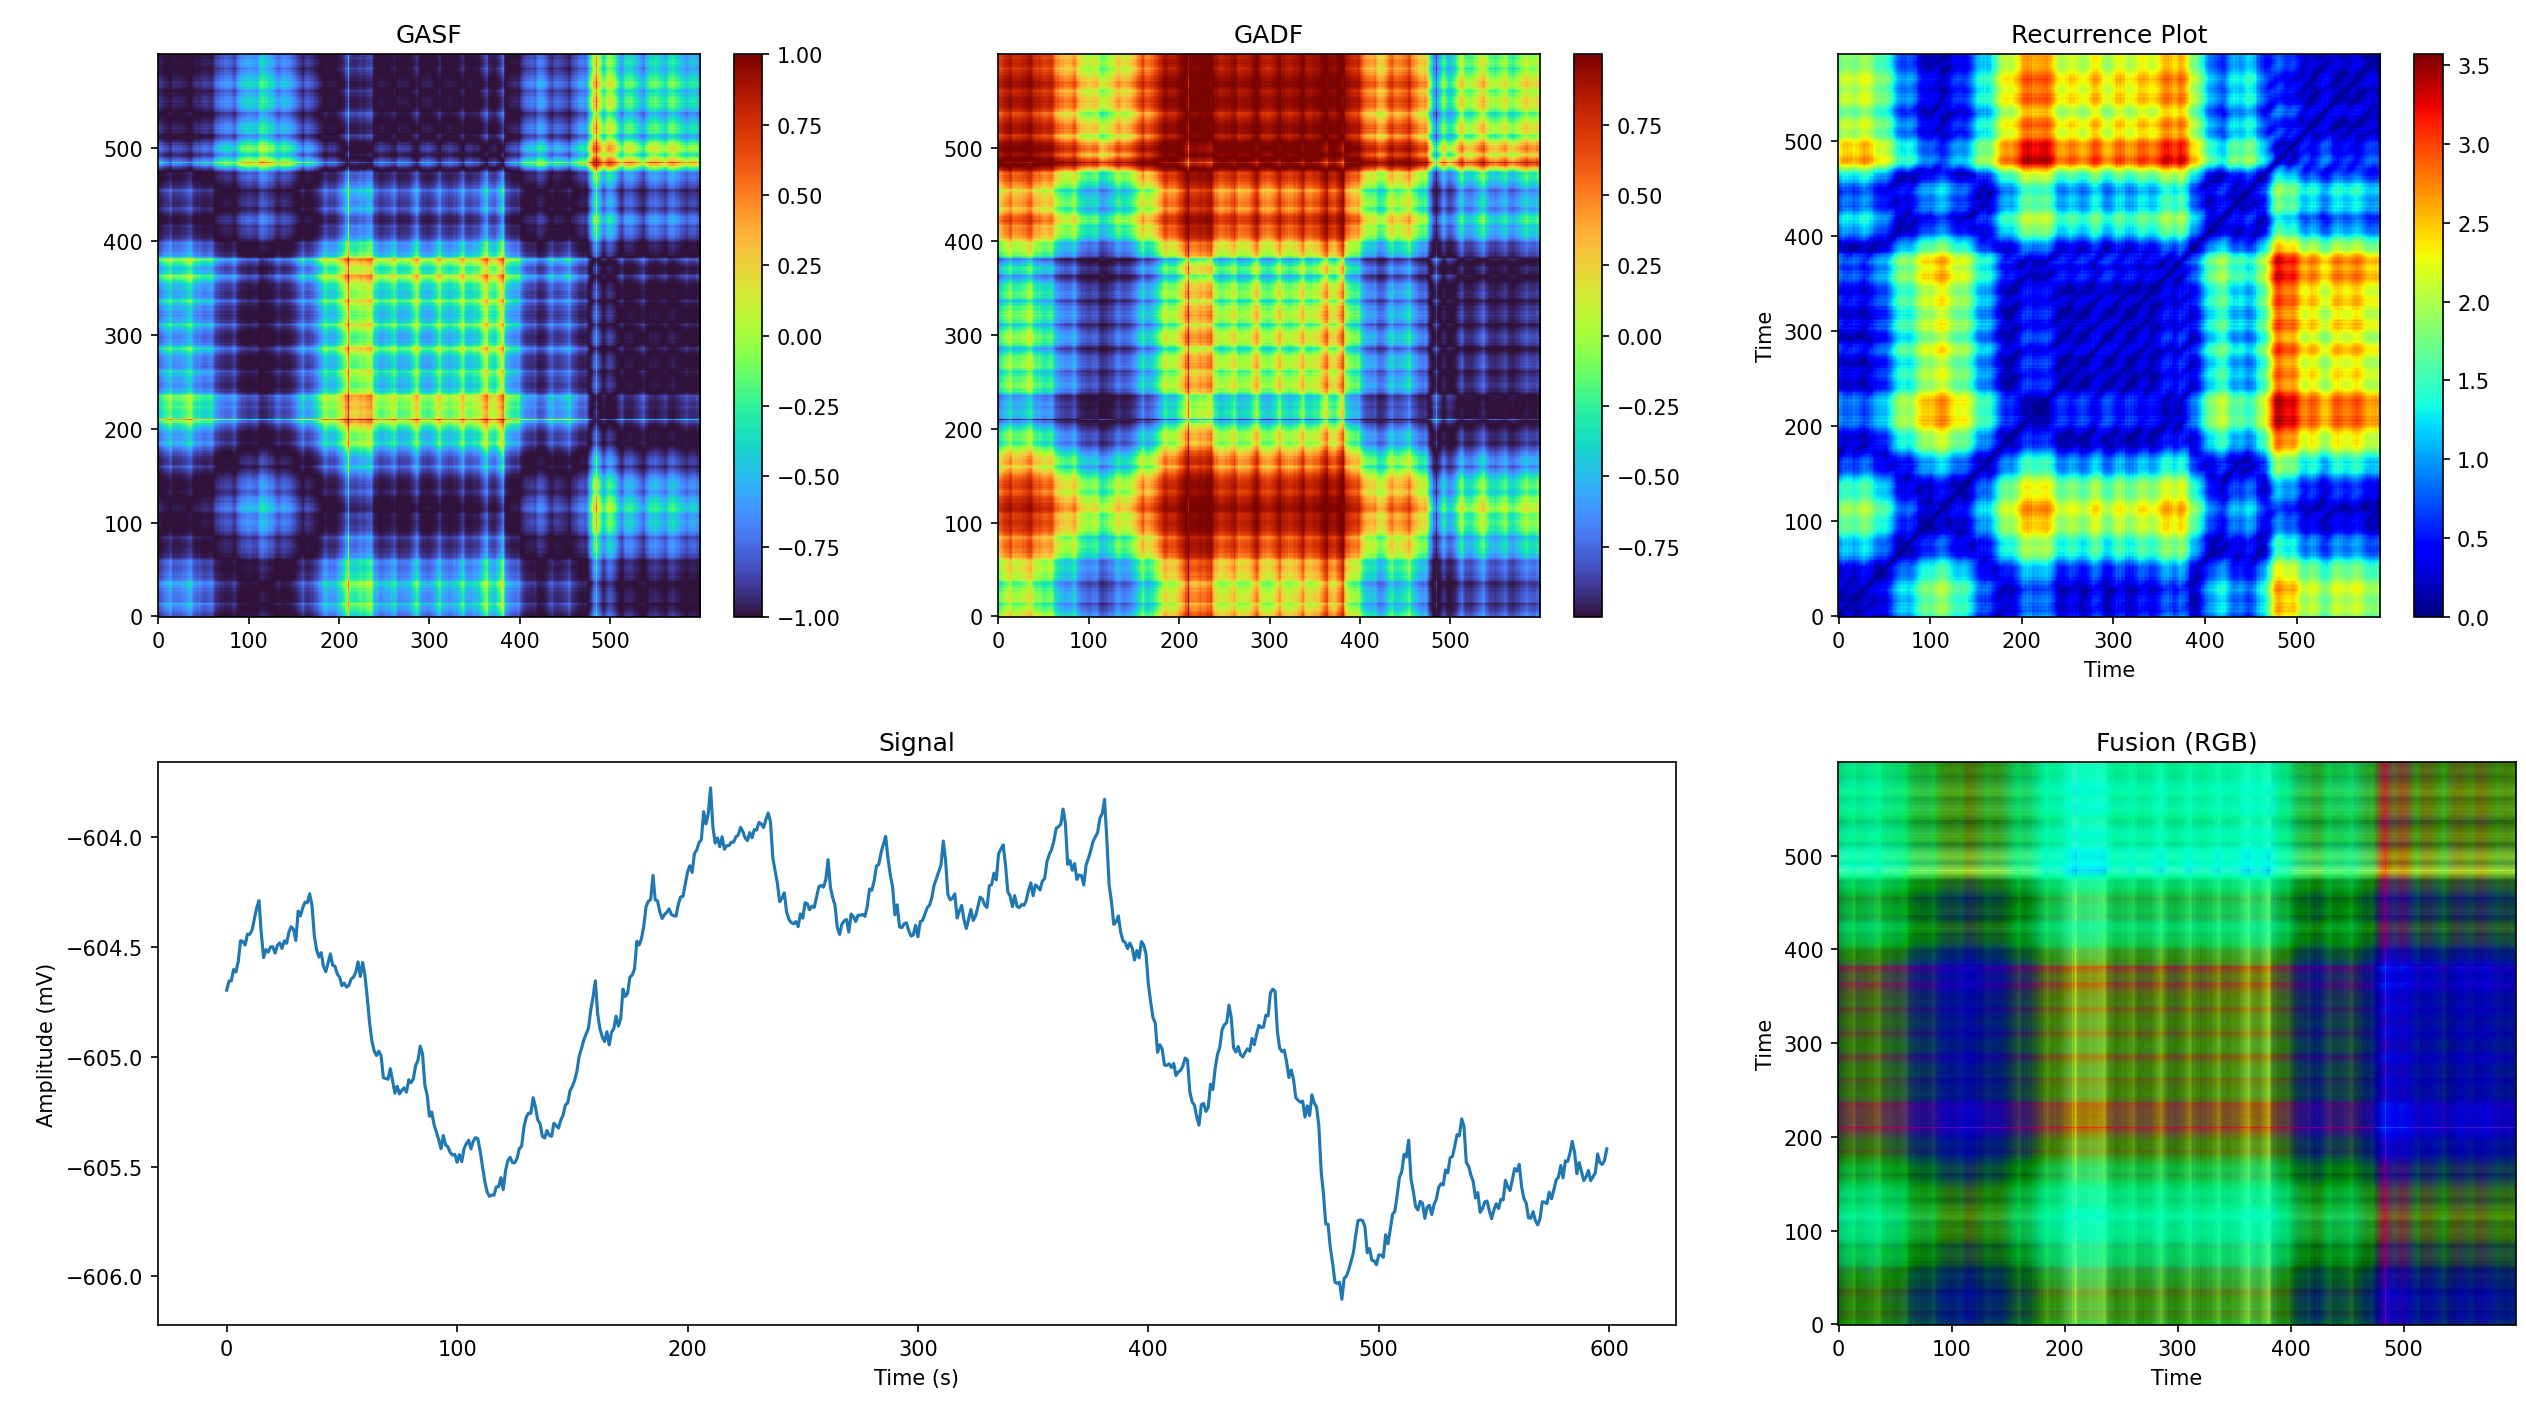
\includegraphics[width=\textwidth]{encodings/cnn_eg.png}
\caption{One 600-second window encoded as a GASF, a GADF, a recurrence plot and their RGB fusion, the four inputs of the CNN models.}
\label{fig:encodings}
\end{figure}

\begin{instructions}
This is the earlier hand-saved figure (\src{Plots/Classification/gramian/cnn_eg.png}). Either redraw it with the
poster's colour scale from \src{Plots/poster/make_panels.py}, or use the cleaner models schematic
(\src{figures/poster/models.png}).
\end{instructions}

\section{Distance, normalisation and scale invariance}
\label{sec:distance}

Every method in this thesis that groups, matches or retrieves a subsequence does so by way of a distance function, and the choice of that function determines what the method is capable of considering ``the same shape''. This section states the distances used and what each is invariant to, because RQ3 is precisely a question about invariance.

For two subsequences $Q = q_1,\ldots,q_m$ and $C = c_1,\ldots,c_m$ of equal length $m$, the Euclidean distance is
\begin{equation}
d(Q,C) = \sqrt{\sum_{i=1}^{m}(q_i - c_i)^2}.
\end{equation}
This is sensitive to both the offset and the amplitude of the two subsequences: a shape occurring during a slow depolarisation drift will be distant from an identical shape occurring at a different baseline, purely because of the offset. Since mycelium recordings exhibit exactly this kind of slow baseline wander, raw Euclidean distance is unsuitable for shape comparison.

The standard remedy is to z-normalise each subsequence before comparison. Writing $\hat{q}_i = (q_i - \mu_Q)/\sigma_Q$ for the mean $\mu_Q$ and standard deviation $\sigma_Q$ of $Q$, the z-normalised Euclidean distance is
\begin{equation}
d_z(Q,C) = \sqrt{\sum_{i=1}^{m}(\hat{q}_i - \hat{c}_i)^2},
\label{eq:znorm}
\end{equation}
which is invariant to offset and to amplitude scaling, and which is the distance the matrix profile is defined over \cite{yeh}. Equation \eqref{eq:znorm} is therefore the default distance throughout this thesis, and where a result is reported against an unnormalised comparison this is stated explicitly.

What Equation \eqref{eq:znorm} is \emph{not} invariant to is duration. Both subsequences must have the same length $m$, and a shape that occurs over four minutes in one region and over twelve minutes in another is not recoverable by a query defined at either length. This matters here more than it does in most domains: multiple scales of oscillatory behaviour are a documented characteristic of these signals \cite{adamatzky2023}, \cite{dehshibi}, and the same morphology has been observed by eye at durations differing by an order of magnitude. Three families of approach address this:

\begin{itemize}
  \item \textbf{Elastic distances}, of which Dynamic Time Warping is the canonical example, allow a non-linear alignment between the time axes of $Q$ and $C$, and so tolerate local stretching and compression. They are more expensive than Equation \eqref{eq:znorm} and admit alignments that are not always physically meaningful.
  \item \textbf{Resampling and uniform scaling}, in which the query is resampled to a range of candidate lengths and the best match across that range is retained. This is conceptually the simplest and is directly compatible with the matrix profile machinery, at the cost of a linear increase in computation with the number of scales searched.
  \item \textbf{Symbolic encodings} such as Symbolic Aggregate Approximation (SAX) \cite{lin2007sax}, which reduce a window to a short string of symbols via piecewise aggregate approximation followed by breakpoint quantisation of the z-normalised amplitude. Because the number of segments is fixed rather than the number of samples, the representation is intrinsically length-agnostic, and comparison becomes a string distance rather than a numerical one. A directional variant (dSAX) encodes the sign of change per segment (up, same, down). A pattern such as \texttt{U+ S? D+} then finds sharkfin-shaped events at any duration.
\end{itemize}

The architectural position taken in this thesis is that \emph{scale is a property of a motif, not of the analysis that discovered it}: every span carries its native duration, and every encoding declares whether or not it is scale-normalised. Whether a motif recurs at other scales is then a query that can be asked of the library, rather than an assumption baked into how the library was built.

\begin{instructions}
Settle the plan's open note on which scale-invariant distance is used. What the project ended with:
\begin{itemize}
  \item seeded search uses $d_z$ at the seed's own length;
  \item the Library offers four distances, including MPdist \cite{gharghabi2018mpdist} and a scale-invariant
        (resampled) distance;
  \item the RQ3 pilot banks searches at 0.8$\times$, 1$\times$ and 1.25$\times$;
  \item the drop-motif study resamples each event to a 200-point frame in units of its own fall.
\end{itemize}
Then state the key finding, which belongs here as theory and in Chapter~\ref{ch:events} as evidence: resampling to a
fixed length removes absolute duration and amplitude but not measurement resolution. The normalised vector still
predicts how many samples an event was built from, at 0.753 balanced accuracy against a chance of 0.25
(\src{Plots/drop_motifs10/CLAIMS.md}, row 9). Normalisation is therefore not the same as invariance.
\end{instructions}

\section{Surrogate data and null hypothesis testing}
\label{sec:surrogates}

A motif discovery algorithm applied to any sufficiently long signal will return motifs. The matrix profile in particular is guaranteed to return the most similar pair of subsequences in a dataset, whether or not that pair is meaningfully similar --- the guarantee is on optimality of the search, not on significance of the result. Reporting that recurring structure was found is therefore not by itself evidence that the signal contains structure. What is required is a null: how much structure of this kind does the same method recover from a signal that is known to contain none of the structure of interest, but is otherwise comparable?

Surrogate data testing supplies that null \cite{theiler1992surrogate}. A surrogate is a synthetic series generated from the original recording so as to preserve certain statistical properties while destroying others. Comparing a statistic computed on the original against the distribution of the same statistic computed on an ensemble of surrogates gives a test of the specific hypothesis that the surrogate generation was designed to destroy.

Three surrogate types are used in this thesis.

\textbf{Phase-randomised surrogates} preserve the power spectrum, and therefore the linear autocorrelation structure, while destroying the phase relationships that give rise to specific waveform shapes. Given a recording $x$ of length $n$, the discrete Fourier transform $X_k$ is computed, the phase of each coefficient is replaced by a value drawn uniformly from $[0, 2\pi)$ subject to conjugate symmetry, and the inverse transform is taken:
\begin{equation}
\tilde{x} = \mathcal{F}^{-1}\!\left\{ |X_k| \, e^{i\phi_k} \right\}, \qquad \phi_k \sim U[0,2\pi).
\end{equation}
The result has the same spectrum and the same autocorrelation as the original, and is a linear Gaussian process in every other respect. A motif recovered from the original but not from its phase-randomised surrogate is therefore evidence of structure that is not explained by the signal's spectral content alone --- which is the relevant null for this project, since slow drifts and broad oscillatory content are known to be present and are not what is being claimed.

\textbf{Amplitude-adjusted (AAFT) surrogates} \cite{theiler1992surrogate,schreiber2000surrogate} also preserve the recording's distribution of values, by rank-remapping a phase-randomised Gaussian series onto the original amplitudes. They are the right null for value-reading measures such as multiscale entropy, where a phase-randomised surrogate would differ from the original in its amplitude distribution as well as its structure.

\textbf{Block-shuffled surrogates} preserve short-range structure within blocks while destroying the ordering between them. The recording is partitioned into contiguous blocks and the blocks are randomly permuted. This provides a complementary null for questions concerning the arrangement of events in time --- such as whether events recur at intervals that are themselves structured --- where phase randomisation would be too destructive to be informative.

In every case, the surrogate is not a different experiment. The identical analytical chain is rerun on the surrogate at identical parameters, and the comparison reported is between two runs of the same recipe. This is implemented in \tool{} as a \texttt{Signal $\rightarrow$ Signal} block (Section~\ref{sec:types}), precisely so that the comparison is cheap enough to run routinely. Figure~\ref{fig:nullviolin} shows a worked example.

\begin{figure}[htbp]
\centering
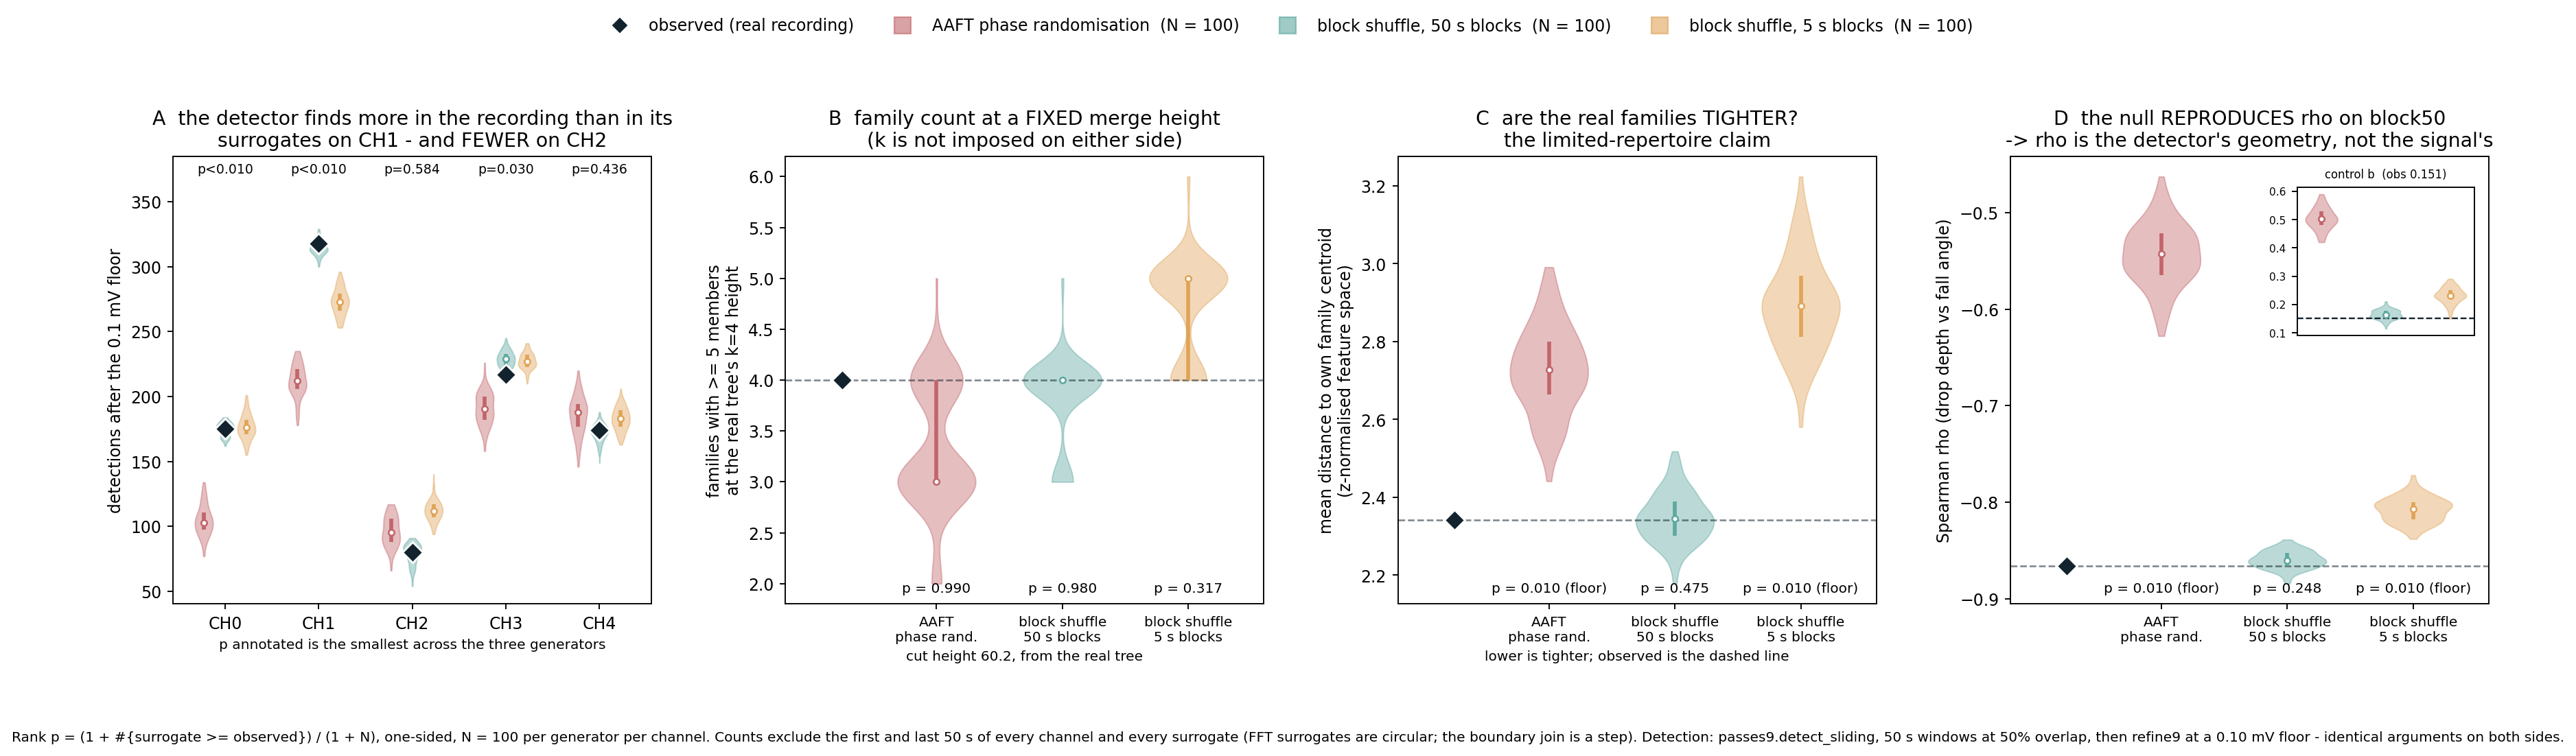
\includegraphics[width=\textwidth]{drop_motifs/NULL_surrogate.png}
\caption{A worked surrogate test from the drop-motif study: observed statistics (detection count, family count, tightness, rank correlation) against AAFT and block-shuffled surrogates.}
\label{fig:nullviolin}
\end{figure}

\begin{instructions}
Settle the plan's two open decisions here.

Realisation counts, as actually used:
\begin{itemize}
  \item 1 draw per task in the detector sweep (cost; 20-draw re-runs on rangpur were prepared);
  \item 20 draws for the demonstration detector;
  \item 200 phase-randomised draws per channel for seed searches;
  \item 3--5 for Library quiet-window nulls;
  \item 200 label shuffles for every classifier null.
\end{itemize}
State the $p$-value floor, $1/(N+1)$: 0.005 at 200 draws. Coverage: 2,587 of 2,936 real runs carry at least one
surrogate, so ``every result'' is true of the reported results, not of every run ever made.

Reporting: rank-based $p$-values plus an effect size, either the real/surrogate ratio or a $z$ against the null
distribution.

Also say what a surrogate is never allowed to be: a detection counted as a finding
(\src{tests/test_surrogate_never_a_detection.py}).
\end{instructions}

\section{Random-convolution classifiers}
\label{sec:minirocket}

\begin{instructions}
New section, about half a page. MiniRocket \cite{dempster2021minirocket} transforms a series with a fixed set of 84
convolution kernels of length 9 (weights from $\{-1, 2\}$), each applied at a range of dilations so that one kernel can
see 9 consecutive samples or a pattern spread over a minute or more. Each kernel--dilation pair is given biases taken
from the data's own quantiles, and contributes one feature: the proportion of positive values (PPV) of its convolution
output.
\begin{itemize}
  \item About 10,000 features result; none is learned.
  \item A ridge classifier is fitted on top. Here it is class-balanced, and Platt scaling \cite{platt1999} maps its
        score to a probability.
  \item In R4 the series is the detected span plus 25\,\% context each side, reduced to 512 points by bin means and
        z-normalised. Four scale features (log duration, peak-to-peak, noise, and their ratio) are appended.
\end{itemize}
Check the exact feature count in \src{DATA/derived/models/rq1b_minirocket/20261020-2343/manifest.json}.
\end{instructions}

\section{Evaluation statistics}
\label{sec:stats}

\begin{instructions}
New section, about one page. Define each statistic once, with the formula and a one-line ``what it answers'':
\begin{itemize}
  \item Precision $=\mathrm{TP}/(\mathrm{TP}+\mathrm{FP})$, the share of a detector's candidates you judged real, with a
        Wilson 95\,\% interval \cite{wilson1927}.
  \item Stratified estimation: the share real across a table of candidate events, estimated from a stratified sample
        weighted by stratum size, with a bootstrap interval \cite{efron1979bootstrap} (1,000--2,000 resamples).
  \item AUC, the probability that a real event outscores a non-event. It does not depend on a cut.
  \item Balanced accuracy, the mean of sensitivity and specificity, robust to the 80:20 imbalance of the 10-minute labels.
  \item Macro F1.
  \item Cohen's $\kappa$ \cite{cohen1960kappa}, for your re-test agreement.
  \item Label-shuffle permutation nulls (labels permuted within recording and kind, the whole fit repeated).
  \item Leave-one-recording-out cross-validation.
  \item Cramér's V \cite{cramer1946}, for family-by-label association.
  \item The cophenetic correlation \cite{sokal1962cophenetic}, for how faithfully a Ward tree \cite{ward1963}
        summarises its distances.
  \item Newcombe's interval for a difference of proportions \cite{newcombe1998} and Fisher's exact test (blind panel).
\end{itemize}
Note why accuracy is not reported alone: a model that always answers ``not interesting'' scores about 0.79--0.81
accuracy on the 10-minute labels.
\end{instructions}
